\documentclass[10pt,twocolumn,letterpaper]{article}

\usepackage{cvpr}
\usepackage{times}
\usepackage{epsfig}
\usepackage{graphicx}
\usepackage{amsmath}
\usepackage{amssymb}
\usepackage{booktabs}
\usepackage{multirow}

\makeatletter
\def\@maketitle{%
   \newpage \null
   \vskip .15in
   \begin{center}
      {\Large \bf \@title \par}
      \vspace*{12pt}
      {\large \lineskip .5em
       \begin{tabular}[t]{c}\@author\end{tabular}\par}
      \vskip .3em
   \end{center}%
}
\makeatother

% Include other packages here, before hyperref.
\usepackage[breaklinks=true,bookmarks=false]{hyperref}

\cvprfinalcopy % *** Uncomment this line for the final submission

\def\cvprPaperID{****}
\def\httilde{\mbox{\tt\raisebox{-.5ex}{\symbol{126}}}}

\setcounter{page}{1}
\begin{document}

%%%%%%%%% TITLE
\title{Decoupling What from Where: Action-Type-Conditioned Grounding for GUI Agents}

\author{
\begin{tabular}{cc}
\begin{tabular}{c}
\textbf{Aadi Chauhan*}\\
Stanford University\\
{\tt\small aadic@stanford.edu}
\end{tabular}
&
\begin{tabular}{c}
\textbf{Arthur Ilyasov*}\\
Stanford University\\
{\tt\small ailyasov@stanford.edu}
\end{tabular}
\end{tabular}
}

\maketitle

%%%%%%%%% ABSTRACT
\begin{abstract}
GUI agents must jointly predict an action type (\emph{click}, \emph{scroll}, \emph{type}, \ldots) and a spatial target coordinate from a single screenshot and instruction. Existing end-to-end vision-language-action models entangle these decisions in one autoregressive decode, producing the documented failure mode of \emph{coherent-but-wrong} grounding: the model commits to an incorrect action type and then grounds precisely within that wrong semantics. We study whether explicitly factoring action-type prediction from spatial grounding reduces this error. Our pipeline runs a frozen Qwen2-VL-2B backbone through a lightweight MLP classifier (Stage~1), then conditions a LoRA-fine-tuned grounding model (Stage~2) on the predicted action-type signal. We evaluate five conditioning mechanisms — flat baseline (A), auxiliary loss (B), hard routing (C), additive embedding hook (D-hook), and prepended learned embedding token (D-token) — across two benchmarks (AITW and Mind2Web) with paired-bootstrap significance. The broad factorization thesis is \textbf{supported}: variants B and D-hook each significantly outperform the flat baseline on spatially informative action types (hit@0.10: $0.305 \pm 0.012$ and $0.300 \pm 0.028$ vs.\ $0.255 \pm 0.021$; $p < 0.002$), and a full two-stage pipeline with predicted types beats the flat baseline end-to-end ($0.271$ vs.\ $0.255$ hit@0.10). The specific architectural claim — that a \emph{learned prepended action-type embedding} is the mechanism — is \textbf{refuted}: a plain auxiliary training loss (B) is the best conditioned variant, and the hypothesized token (D-token) does not reach B/D-hook on headline metrics. A M-RoPE implementation pitfall that silently produces an $8\sigma$ false negative is documented and corrected. Conditioning advantage is largest at low data ($n=300$: $+0.067$ hit@0.10) and concentrated in the \emph{click} class, revealing that the gain is click-vs-scroll/type disambiguation rather than field localization.
\end{abstract}

%%%%%%%%% BODY TEXT
\section{Introduction}

A GUI agent maps a screenshot and a natural-language instruction to a low-level action: a type (\emph{click}, \emph{scroll}, \emph{type}, \emph{drag}, \emph{hotkey}, \ldots) and, for spatial actions, a pixel-level target. State-of-the-art native agents — UI-TARS~\cite{uitars}, OS-Atlas~\cite{osatlas}, SeeClick~\cite{seeclick}, ShowUI~\cite{showui} — emit both in one autoregressive token stream from the same head, treating action type and location as an entangled prediction problem.

This design has a documented failure mode. When the model commits to an incorrect action type — scrolling past a visible target instead of clicking it, typing into a button rather than an input field — it then grounds \emph{coherently} within that incorrect semantic frame, producing an action that is locally consistent but globally wrong. On long-horizon tasks, these errors compound: each mistyped action changes screen state in a way that makes subsequent actions harder. Mind2Web's official metrics already separate element accuracy, operation F1, and step success rate, reflecting that getting the type right and getting the location right are distinct sub-problems~\cite{mind2web}.

\begin{figure}[t]
\begin{center}
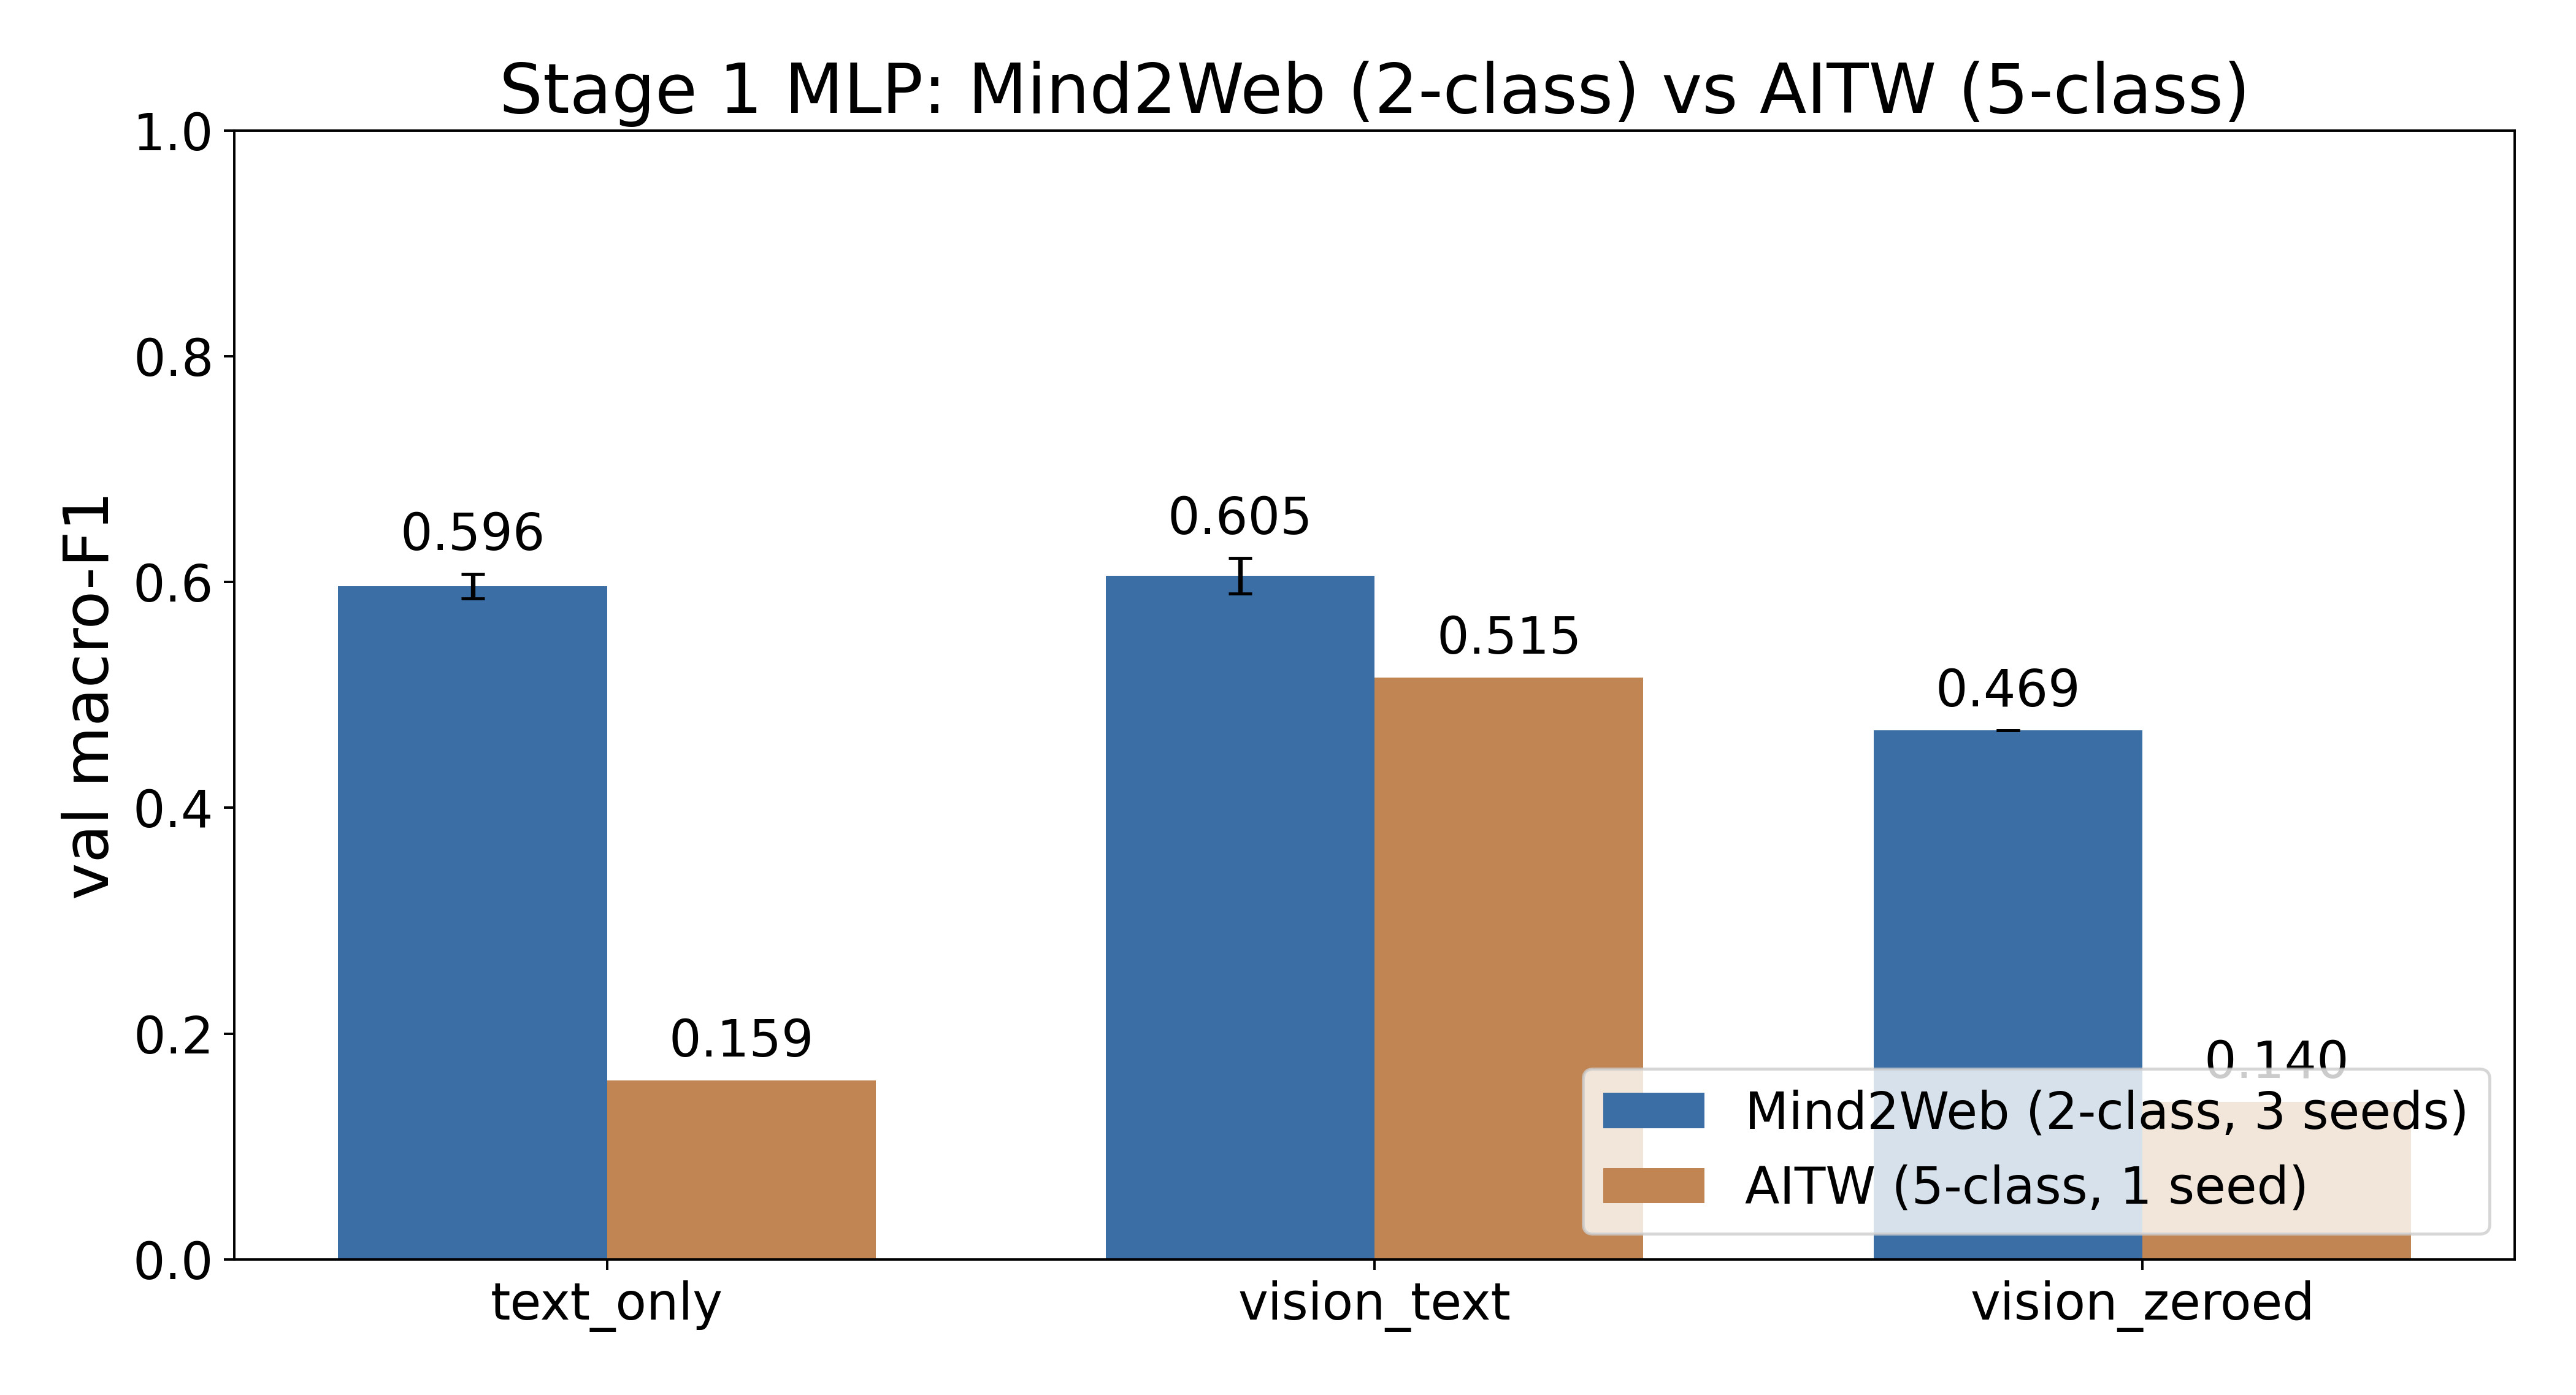
\includegraphics[width=0.98\linewidth]{figures/stage1_mind2web_vs_aitw.png}
\end{center}
\caption{Stage 1 action-type classifier macro-F1 on Mind2Web (2 active classes) and AITW (5 active classes). Vision is essential on AITW ($+0.414$ over text-only) but redundant on Mind2Web ($+0.009$), because AITW instructions describe \emph{goals} rather than physically specifying the action.}
\label{fig:stage1_comparison}
\end{figure}

We study whether explicitly factoring action-type prediction from spatial grounding helps. Our two-stage pipeline is:
\begin{enumerate}
\item \textbf{Stage~1.} A frozen Qwen2-VL-2B encoder produces mean-pooled hidden-state features; a 3-layer MLP classifies the action type from these features.
\item \textbf{Stage~2.} A LoRA-fine-tuned Qwen2-VL-2B grounding model receives the predicted action type as an additional conditioning signal and produces a coordinate string.
\end{enumerate}

We evaluate five conditioning mechanisms for Stage~2 and report the following findings:

\begin{itemize}
\item \textbf{Broad thesis supported.} Action-type supervision significantly improves grounding when action type is spatially informative (click-vs-scroll/type). The effect vanishes on a matched control where action type is not spatially predictive.
\item \textbf{Specific claim refuted.} The hypothesized mechanism — a learned prepended action-type embedding — is not the best conditioned variant. A plain auxiliary training loss captures the full benefit more simply.
\item \textbf{Mechanism identified.} The gain is concentrated in the \emph{click} class; the \emph{type} class is ungroundable on AITW due to degenerate coordinates, so the real signal is click-vs-other disambiguation.
\item \textbf{Implementation pitfall documented.} Injecting action conditioning via \texttt{inputs\_embeds} bypasses Qwen2-VL's M-RoPE position computation, producing an 8$\sigma$ false negative if uncorrected.
\end{itemize}

\section{Related Work}

\textbf{End-to-end GUI agents.} The dominant paradigm treats action type, arguments, and coordinates as one autoregressive output. UI-TARS~\cite{uitars} exemplifies this with a unified action space across platforms and explicit thought traces. OS-Atlas~\cite{osatlas} scales the same paradigm with 13M cross-platform GUI grounding instances and shows that action-label harmonization across web/Android/desktop is nontrivial. ShowUI~\cite{showui} builds a compact VLA around Qwen2-VL with interleaved vision-language-action streaming. Our flat baseline (Variant~A) directly replicates the joint-decoding paradigm of these systems.

\textbf{Modular grounding.} SeeClick~\cite{seeclick} argues that grounding is the central bottleneck in visual GUI agents and shows that continual grounding pre-training correlates with downstream agent gains. UGround / SeeAct-V~\cite{uground} separates planning from grounding at the text-vs-pixel boundary, using a dedicated visual grounding model for coordinate prediction. GUI-Actor~\cite{guiactor} replaces coordinate-token regression with an attention-based action head driven by a dedicated \texttt{<ACTOR>} token plus a verifier, achieving 44.6 on ScreenSpot-Pro. Our work differs: the module boundary we study is between \emph{action-type prediction} and \emph{spatial grounding}, not between planning text and coordinates.

\textbf{Reward decomposition.} UI-R1~\cite{uir1} applies RL fine-tuning with a rule-based reward that explicitly separates action-type accuracy from action-argument accuracy, reporting $+15$ points in action-type accuracy and $+10.3$ in grounding over the base model on AndroidControl. This is the closest training analog: like our project, it treats type and location as separable optimization targets. Our approach differs in using supervised conditioning rather than RL.

\textbf{Test-time grounding refinement.} RegionFocus~\cite{regionfocus} achieves large ScreenSpot-Pro gains through training-free iterative zoom and image-as-map landmarks. Our work is orthogonal: we change the conditioning pathway at training time rather than refining at inference.

\textbf{Modular decision-making foundations.} SayCan~\cite{saycan} separates ``useful according to language'' from ``feasible according to the environment'' in robotics, providing a conceptual precedent for our action-type / grounding split. ReAct~\cite{react} motivates explicit intermediate variables between reasoning and acting. RT-2~\cite{rt2} is the reference for unified token-level action generation — the paradigm we critically examine.

\section{Data}

\textbf{Sources.} We use two datasets unified under a canonical 8-class action taxonomy: \emph{click}, \emph{double\_click}, \emph{type}, \emph{scroll}, \emph{drag}, \emph{hotkey}, \emph{wait}, \emph{finished}.

\textbf{Mind2Web}~\cite{mind2web} provides $\sim$137k web interaction steps from 2,350 tasks across 137 real websites, in multimodal form via the \texttt{osunlp/Multimodal-Mind2Web} release. We use the \texttt{train} split (7,775 steps) for Stage~1 MLP training and \texttt{test\_task} (1,338 steps) for evaluation. The dataset has a strong click majority ($\sim$88\%) and only two active classes at meaningful scale (click, type), making it useful for a cross-dataset control but insufficient as the primary multi-class benchmark.

\textbf{Android in the Wild (AITW)}~\cite{aitw} provides $\sim$715k episodes of Android interaction, available via the \texttt{cjfcsjt/AITW\_General} HuggingFace mirror. We use 5,000 training steps and 1,000 validation steps for Stage~1, and $n_{\text{train}} \in \{300, 500, 800, 1200, 2500, 5000\}$ for Stage~2 ablation studies. AITW provides five active canonical classes (click 55\%, scroll 13\%, finished 12\%, type 11\%, hotkey 9\%) with richer action diversity than Mind2Web.

\textbf{Preprocessing.} Mind2Web canonical mapping is straightforward (CLICK, TYPE, SELECT all map through the taxonomy). AITW presents two non-trivial issues:

\emph{Raw image decoding.} AITW screenshots are stored as raw RGB pixel bytes with no PNG/JPEG header. We implement \texttt{\_decode\_aitw\_image\_bytes} to handle seven observed $(w, h)$ shapes (540$\times$1080, 540$\times$1140, 540$\times$1170, 720$\times$1520, 720$\times$1440, 412$\times$732, 270$\times$600) plus a portrait-aspect fallback guesser, rather than calling \texttt{PIL.Image.open()} which raises \texttt{UnidentifiedImageError}.

\emph{DUAL\_POINT action splitting.} AITW stores most actions as \texttt{DUAL\_POINT} with touch and lift coordinates. We split into \emph{tap} (mapped to click) vs.\ \emph{swipe} (mapped to scroll) using the Euclidean distance between touch and lift normalized to image dimensions, with threshold 0.04.

\emph{Class-balanced sampling.} To address the $\sim$80\% click majority in both datasets, Stage~2 training uses a class-balanced sampler that draws $n_{\text{per\_class}}$ examples from each canonical action, bootstrap-sampling minority classes.

\textbf{Coordinate format.} Ground-truth spatial targets are normalized to $[0, 1]$ and converted to the string \texttt{``(x, y)''} with integer values in $[0, 999]$, providing fixed-length targets for autoregressive token prediction.

\section{Methods}

Our pipeline has two stages. Below we describe each in turn, then detail the five conditioning variants evaluated in Stage~2.

\subsection{Stage 1: Action-Type Classifier}

We extract features from a \emph{frozen} Qwen2-VL-2B-Instruct~\cite{qwen2vl} backbone. Given a screenshot and instruction formatted as a chat prompt, we run a forward pass and mean-pool the final hidden states across all unmasked tokens, producing a 1536-dim vector per example. Two modes are evaluated: \texttt{text\_only} (instruction + target HTML, no image) and \texttt{vision\_text} (instruction + HTML + screenshot).

A 3-layer MLP (1536 $\to$ 1024 $\to$ 256 $\to$ 8) is trained on these cached features with class-weighted cross-entropy, AdamW ($\text{lr}=10^{-4}$, $\text{wd}=0.01$), batch size 128, and 8 epochs, selecting the best checkpoint by validation macro-F1.

\subsection{Stage 2: Action-Type-Conditioned Grounding}

Stage~2 fine-tunes Qwen2-VL-2B with LoRA (rank 16, applied to query/key/value/output projections) to produce coordinate string \texttt{``(x, y)''} given the screenshot, instruction, and (for conditioned variants) the predicted action type. Loss is computed only on the coordinate tokens; image and instruction tokens are masked with $-100$.

We evaluate five variants, each sharing identical data, optimizer ($\text{lr} = 2 \times 10^{-5}$), and evaluation harness. The only difference is how action-type information is incorporated:

\textbf{A (flat baseline).} No action-type conditioning. Prompt: \texttt{[screenshot] [instruction] → (x, y)}. This replicates the standard joint end-to-end decoding paradigm.

\textbf{B (auxiliary loss).} Adds a linear action-type classification head on top of the LoRA model's pooled representation. Training jointly minimizes grounding loss and action-type cross-entropy. \emph{No action-type information is provided at inference time.}

\textbf{C (hard routing).} The model is trained to emit the action-type word before the coordinate: \texttt{``click (x, y)''}. At inference, the gold (or predicted) action-type word is forced as a decode prefix, and non-matching tokens are masked from the logits.

\textbf{D-hook (additive embedding).} A learned action-type embedding table $E \in \mathbb{R}^{8 \times d}$ provides one embedding per class. At each forward pass, the embedding for the predicted action type is added to all token embeddings via a forward hook on the embedding layer. Conditioning is diffuse (embedding norm $\approx 0.06$) and preserves the normal \texttt{input\_ids} path.

\textbf{D-token (prepended token, the hypothesis).} A dedicated sentinel token \texttt{<|action\_slot|>} is appended to the tokenizer vocabulary. During training and inference, this token is prepended to the instruction, and its embedding is replaced in-place with the row of $E$ corresponding to the current action type. Because the token is in the normal \texttt{input\_ids} path, Qwen2-VL's M-RoPE position computation is preserved. The embedding norm at convergence is $\approx 2.2$, making the conditioning signal routable and localized.

\paragraph{Training objective.}
Let $s$ be the screenshot, $g$ the instruction, $a \in \{1,\dots,8\}$ the action type, and $y_{1:T}$ the ground-truth coordinate token string. Every variant minimizes the autoregressive grounding loss, computed only over coordinate tokens,
\begin{equation}
\mathcal{L}_{\mathrm{coord}} = -\sum_{t=1}^{T} \log p_\theta\!\big(y_t \mid y_{<t},\, s,\, g,\, c\big),
\label{eq:coord}
\end{equation}
where $c$ is the variant-specific conditioning. The flat baseline (A) uses $c=\varnothing$. The auxiliary-loss variant (B) adds a linear head $h_\phi$ on the mean-pooled hidden state $\bar{z}$ and minimizes
\begin{equation}
\mathcal{L}_{\mathrm{B}} = \mathcal{L}_{\mathrm{coord}} + \lambda\,\mathrm{CE}\!\big(h_\phi(\bar{z}),\, a\big), \qquad \lambda = 1,
\label{eq:aux}
\end{equation}
with no conditioning at inference ($c=\varnothing$). The embedding variants set $c = E[a]$, the learned row of $E$, injected additively across all token embeddings (D-hook) or substituted at the slot position (D-token); both optimize Eq.~\eqref{eq:coord} with $E$ trained jointly by backpropagation. Hard routing (C) appends the action word to the target and optimizes Eq.~\eqref{eq:coord} over the word-plus-coordinate string, forcing the word as a decode prefix at test time.

\paragraph{Implementation.}
Our code builds on HuggingFace Transformers and the PEFT LoRA implementation for the Qwen2-VL-2B backbone; all Stage~1 feature extraction and MLP training, the five Stage~2 conditioning mechanisms, the grounding evaluation and paired-bootstrap harness, and the AITW/Mind2Web preprocessing are our own. Training and feature extraction are orchestrated on Modal (NVIDIA L4 GPUs).

\subsection{M-RoPE Implementation Pitfall}

\begin{figure}[t]
\begin{center}
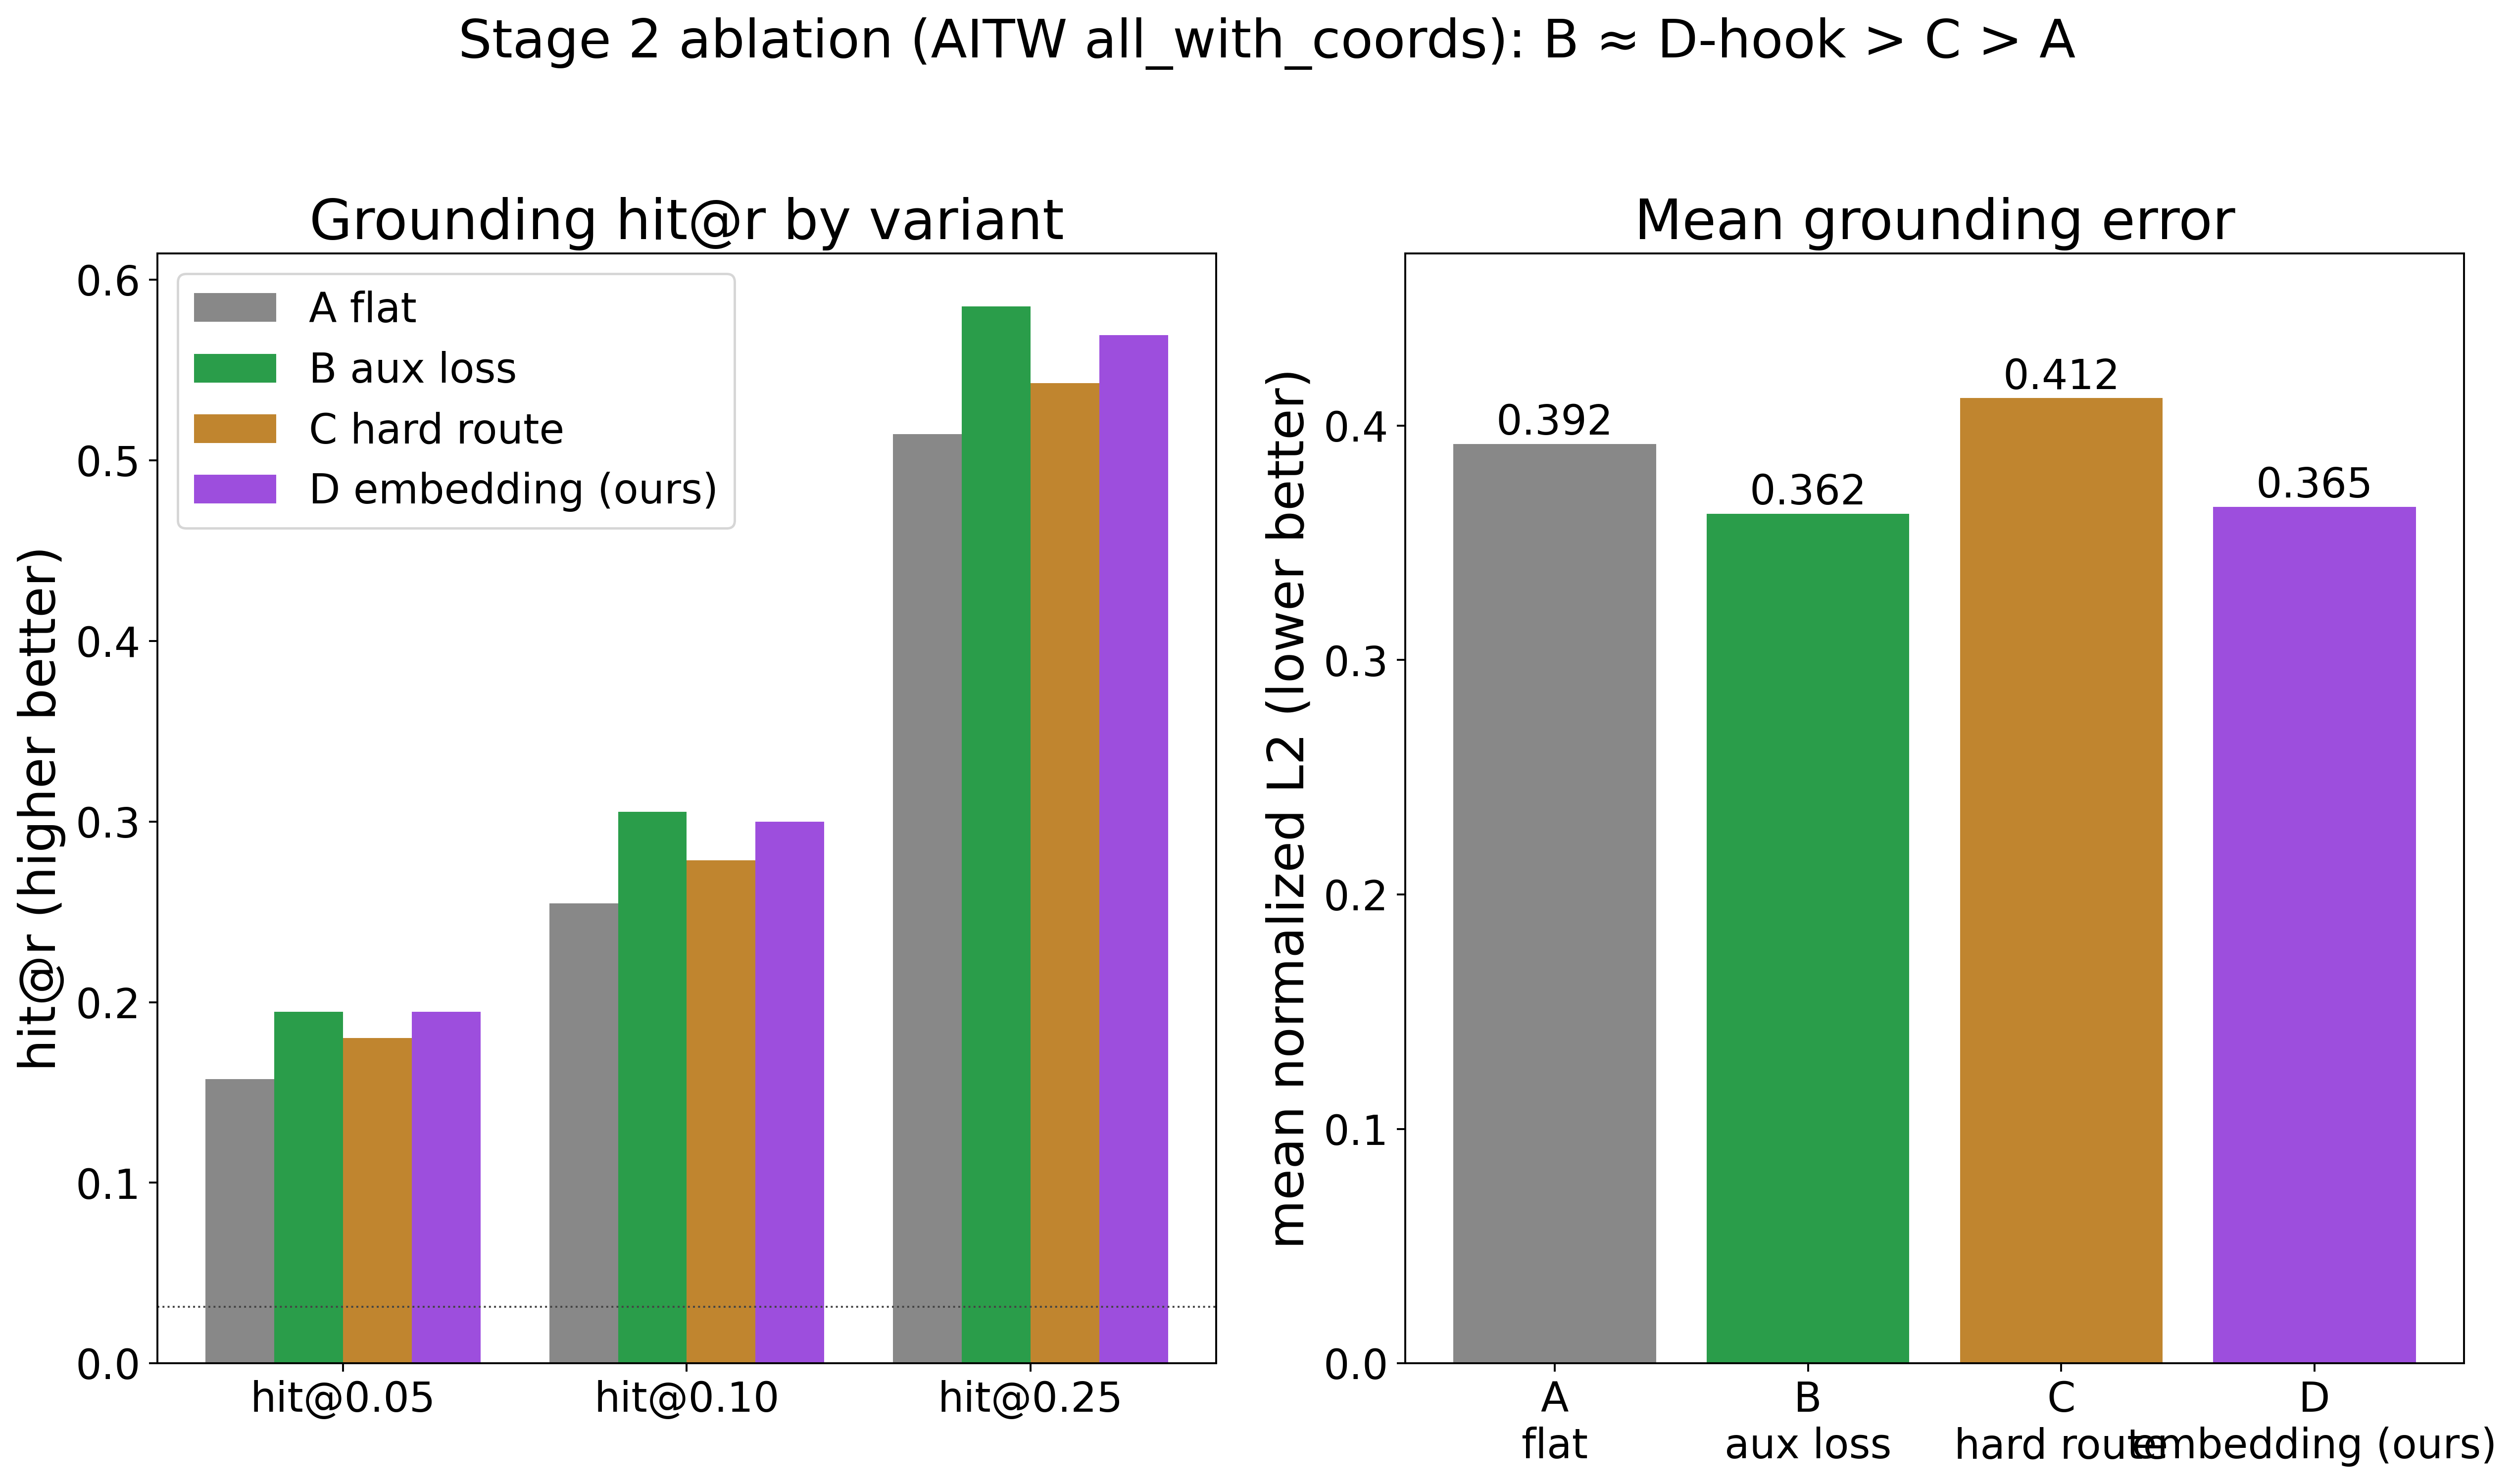
\includegraphics[width=0.98\linewidth]{figures/ablation_ABCD_all_with_coords.png}
\end{center}
\caption{Stage~2 ablation on AITW \texttt{all\_with\_coords} (action type spatially informative). B and D-hook significantly outperform the flat baseline A (paired bootstrap, $p < 0.002$). D-token, the literal hypothesized architecture, does not reach B/D-hook on headline hit@0.10 or hit@0.25.}
\label{fig:ablation}
\end{figure}

Qwen2-VL uses Multimodal Rotary Position Embedding (M-RoPE), which assigns 3D position IDs (temporal, height, width) to visual tokens using the \texttt{input\_ids}-keyed path. An earlier implementation of D-token injected action conditioning via \texttt{inputs\_embeds} directly, bypassing \texttt{input\_ids}. This caused Qwen2-VL's image-token position IDs to be computed without the action slot in the sequence, silently mis-aligning multimodal position embeddings for all visual tokens. The effect was an 8$\sigma$ false negative: Variant~A significantly outperformed the original D, when the correct outcome after fixing is near parity or a D advantage. D-hook and D-token both correct this by preserving the \texttt{input\_ids} path. Practitioners using \texttt{inputs\_embeds} injection with M-RoPE-based models should verify that position-ID computation is unaffected.

\subsection{Evaluation Metrics}

\textbf{hit@$r$}: fraction of predictions whose normalized L2 distance to the ground-truth coordinate is $\leq r$. We report $r \in \{0.05, 0.10, 0.25\}$; the headline metric is hit@0.10.

\textbf{Mean L2}: mean normalized Euclidean distance to the ground truth (lower is better).

\textbf{Paired bootstrap}: significance testing on aligned per-example distances, 1000 bootstrap resamples, $n = 750$ examples per comparison.

\section{Experiments}

All Stage~2 experiments use AITW unless noted. We run 3 seeds (42, 43, 44) for each variant and report mean $\pm$ std. Modal GPU compute (NVIDIA L4) is used for all training and feature extraction.

\subsection{Stage 1: Vision Is Essential on AITW}

\begin{table}[tb]
\begin{center}
\small
\begin{tabular}{lcc}
\toprule
Variant & Mind2Web & AITW \\
 & macro-F1 & macro-F1 \\
\midrule
text\_only & $0.597 \pm 0.011$ & $0.141 \pm 0.032$ \\
vision\_text & $\mathbf{0.605 \pm 0.016}$ & $\mathbf{0.555 \pm 0.036}$ \\
vision\_zeroed & $0.469 \pm 0.000$ & $0.110 \pm 0.051$ \\
\midrule
Vision delta & $+0.009$ & $+0.414$ \\
TF-IDF + LogReg & $0.622$ & $0.168$ \\
Majority floor & $0.472$ & $0.140$ \\
\bottomrule
\end{tabular}
\end{center}
\caption{Stage~1 action-type classifier macro-F1 on Mind2Web (2 active classes) and AITW (5 active classes). Vision contributes minimally on Mind2Web but is decisive on AITW, where instruction text has no action-type-predictive signal.}
\label{tab:stage1}
\end{table}

Table~\ref{tab:stage1} and Figure~\ref{fig:stage1_comparison} show the Stage~1 results. The vision contribution is qualitatively different across benchmarks. On Mind2Web, instructions directly contain action-type words (``click the submit button''), so the screenshot adds only $+0.009$ macro-F1. On AITW, instructions describe user \emph{goals} (``open a new Chrome private window'') with no physically specified action, so text-only features collapse to near-majority-class ($0.141$); vision is decisive ($+0.414$, 40$\times$ larger delta).

The sanity check passes: \texttt{vision\_zeroed} (zero features) collapses to the majority floor, confirming the MLP uses features rather than a class prior. The TF-IDF + LogReg ceiling on AITW is 0.168 (barely above majority), confirming text-only is hopeless on this benchmark regardless of classifier strength.

\subsection{Stage 2 Main Ablation: all\_with\_coords}

The primary ablation uses AITW data where all five action classes are present and coordinates are meaningful: $n_{\text{train}} = 1200$, 2 epochs, \texttt{all\_with\_coords} data mix. Table~\ref{tab:ablation} and Figure~\ref{fig:ablation} show the results.

\begin{table}[tb]
\begin{center}
\small
\begin{tabular}{lccc}
\toprule
Variant & hit@0.10 & hit@0.25 & mean L2 $\downarrow$ \\
\midrule
A (flat) & $0.255 \pm 0.021$ & $0.515$ & $0.392$ \\
B (aux loss) & $\mathbf{0.305 \pm 0.012}$ & $\mathbf{0.585}$ & $\mathbf{0.362}$ \\
C (hard routing) & $0.279 \pm 0.032$ & $0.543$ & $0.412$ \\
D-hook (additive) & $0.300 \pm 0.028$ & $0.569$ & $0.365$ \\
D-token (prepended) & $0.269 \pm 0.025$ & $0.533$ & $0.375$ \\
\bottomrule
\end{tabular}
\end{center}
\caption{Stage~2 ablation on AITW \texttt{all\_with\_coords} ($n_{\text{train}}=1200$, 3 seeds). Paired bootstrap confirms B and D-hook each beat A ($p < 0.002$). D-token does not reach B/D-hook on hit@0.10 or hit@0.25.}
\label{tab:ablation}
\end{table}

Paired bootstrap confirms that \textbf{B and D-hook each significantly outperform A} on all three metrics ($p < 0.002$). \textbf{Ranking: B $\approx$ D-hook $>$ D-token $\gtrsim$ C $>$ A.}

D-token's comparison to A is mixed: it improves hit@0.05 ($+0.027$, $p=0.003$) and mean L2 ($-0.017$, $p<0.001$), but not hit@0.10 ($+0.015$, ns) or hit@0.25 ($+0.019$, ns). Against B, D-token is significantly \emph{worse} on hit@0.10, hit@0.25, and mean L2. The hypothesis that a stronger embedding signal (D-token norm $\approx 2.2$ vs.\ D-hook norm $\approx 0.06$) is better is refuted: a strong localized signal appears to compete with the image/instruction for attention rather than synergize.

C (hard routing) performs middling: it forces the action-type word as a decode prefix, which helps click grounding but derails scroll prediction (Section~\ref{sec:perclass}).

\subsection{Control Condition: taps\_and\_swipes}

\begin{table}[tb]
\begin{center}
\small
\begin{tabular}{lccc}
\toprule
Variant & hit@0.10 & hit@0.25 & mean L2 $\downarrow$ \\
\midrule
A (flat) & $0.390 \pm 0.008$ & $0.727$ & $0.184$ \\
B (aux loss) & $0.368 \pm 0.009$ & $0.730$ & $0.173$ \\
C (hard routing) & $0.325 \pm 0.032$ & $0.635$ & $0.271$ \\
D-hook (additive) & $0.392 \pm 0.035$ & $0.723$ & $0.179$ \\
\bottomrule
\end{tabular}
\end{center}
\caption{Control condition: AITW \texttt{taps\_and\_swipes} ($n_{\text{train}}=1000$). When action type is not spatially informative (taps and swipes both land anywhere on screen), no conditioned variant beats A. D-hook is neutral; C is worse. This confirms the conditioning gain requires a spatially predictive action-type signal.}
\label{tab:control}
\end{table}

Table~\ref{tab:control} shows the \texttt{taps\_and\_swipes} control: only tap (click) and swipe (scroll) actions, where knowing action type carries no information about target location. No conditioned variant beats A. D-hook is neutral ($\Delta \approx 0$), B trades slightly lower hit@0.10 for slightly lower mean L2, and C is worse. This confirms the central prediction: \textbf{action-type conditioning helps if and only if action type is spatially predictive.}

A second control benchmark, Multimodal-Mind2Web (click/type-dominated), replicated this pattern: D-hook vs.\ A yields $-0.006$ hit@0.10 and $+0.018$ hit@0.25 (both near zero), on $n_{\text{train}}=1000$, 2 seeds.

\subsection{End-to-End Pipeline}

\begin{table}[tb]
\begin{center}
\small
\begin{tabular}{lc}
\toprule
Configuration & hit@0.10 \\
\midrule
Flat A baseline & $0.255$ \\
Stage~1 accuracy (val) & $0.843$ \\
Stage~2 oracle (gold types) & $0.292$ \\
\textbf{Stage~2 predicted (Stage~1 types)} & $\mathbf{0.271}$ \\
Oracle $\to$ predicted gap & $0.021 \pm 0.008$ \\
\bottomrule
\end{tabular}
\end{center}
\caption{End-to-end two-stage pipeline on AITW \texttt{all\_with\_coords}. The predicted-type pipeline beats the flat baseline ($0.271 > 0.255$). The oracle-to-predicted gap is small ($0.021$) because Stage~1 is accurate.}
\label{tab:e2e}
\end{table}

Table~\ref{tab:e2e} shows the end-to-end result with Stage~1 predicted types feeding Stage~2. The real two-stage pipeline beats the flat baseline ($0.271 > 0.255$ hit@0.10). The oracle-to-predicted gap is $0.021$, small because Stage~1 achieves 0.843 val accuracy on the 3-class (click/scroll/type) problem in-job. Classifier error is not the bottleneck.

\subsection{Per-Action-Type Decomposition}
\label{sec:perclass}

\begin{figure*}[t]
\begin{center}

\includegraphics[width=0.93\linewidth]{figures/qualitative_grounding.png}
\end{center}
\caption{Qualitative grounding predictions on held-out AITW screenshots: ground truth (green $\circ$), flat baseline A (red $\times$), and conditioned D-hook (blue $\times$); each panel reports both per-example normalized distances. Across \emph{click} and \emph{scroll} examples, the conditioned model (blue) lands nearer the target than the flat baseline (red), consistent with the per-class analysis in Table~\ref{tab:perclass}.}
\label{fig:qualitative}
\end{figure*}

\begin{figure}[t]
\begin{center}

\includegraphics[width=0.98\linewidth]{figures/compounding_error_per_class.png}
\end{center}
\caption{Stage~2 hit@0.10 broken down by action class on \texttt{all\_with\_coords}. The conditioning advantage ($\Delta$ vs.\ A) is concentrated in \emph{click}. The \emph{type} class scores 0.000 across all variants due to degenerate AITW coordinates. The real grounding signal is \emph{click-vs-scroll/type} disambiguation.}
\label{fig:perclass}
\end{figure}

Figure~\ref{fig:perclass} and Table~\ref{tab:perclass} break down Stage~2 hit@0.10 by action class. The overall conditioning win is a \emph{click} win. B gains $+0.120$ and C gains $+0.122$ on click (68\% of the val set), explaining their overall headline improvement. The \emph{type} class scores exactly $0.000$ hit@0.10 across \emph{all} variants, with mean normalized L2 $= \sqrt{2}$ (corner-to-corner), revealing that AITW \texttt{type} actions carry pinned/degenerate touch coordinates that are ungroundable by any model. This corrects an earlier interpretation: the grounding gain is not about localizing text input fields; it is about \emph{click-vs-scroll/type disambiguation} for the precise-target class. Figure~\ref{fig:qualitative} shows representative predictions illustrating this: the conditioned model lands nearer the target than flat A on both click and scroll examples.

\begin{table}[tb]
\begin{center}
\small
\begin{tabular}{lcccc}
\toprule
Action & A & $\Delta$B & $\Delta$D-hook & $\Delta$D-token \\
\midrule
click (68\%) & 0.253 & $+0.120$ & $+0.058$ & $+0.064$ \\
scroll (18\%) & 0.313 & $-0.023$ & $+0.039$ & $-0.016$ \\
type (14\%)   & 0.000 & $0.000$  & $0.000$  & $0.000$ \\
\bottomrule
\end{tabular}
\end{center}
\caption{Per-class hit@0.10 on \texttt{all\_with\_coords}. B and C achieve large click gains ($+0.12$) but diverge on scroll (B small cost; C large loss). D-hook is the only variant that improves both click and scroll.}
\label{tab:perclass}
\end{table}

C's mediocrity is now explained: it has the \emph{largest} click gain ($+0.122$) but \emph{destroys} scroll ($-0.144$), because forcing a decode prefix that conditions the model on ``scroll'' derails the model's spatial reasoning for the gesture class. B captures the click gain ($+0.120$) with only a modest scroll cost ($-0.023$), making it the best overall variant. D-hook uniquely improves both click ($+0.058$) and scroll ($+0.039$), suggesting its diffuse additive signal supports both precise and gestural targets.

\subsection{Data-Scaling Curve}

\begin{figure}[t]
\begin{center}
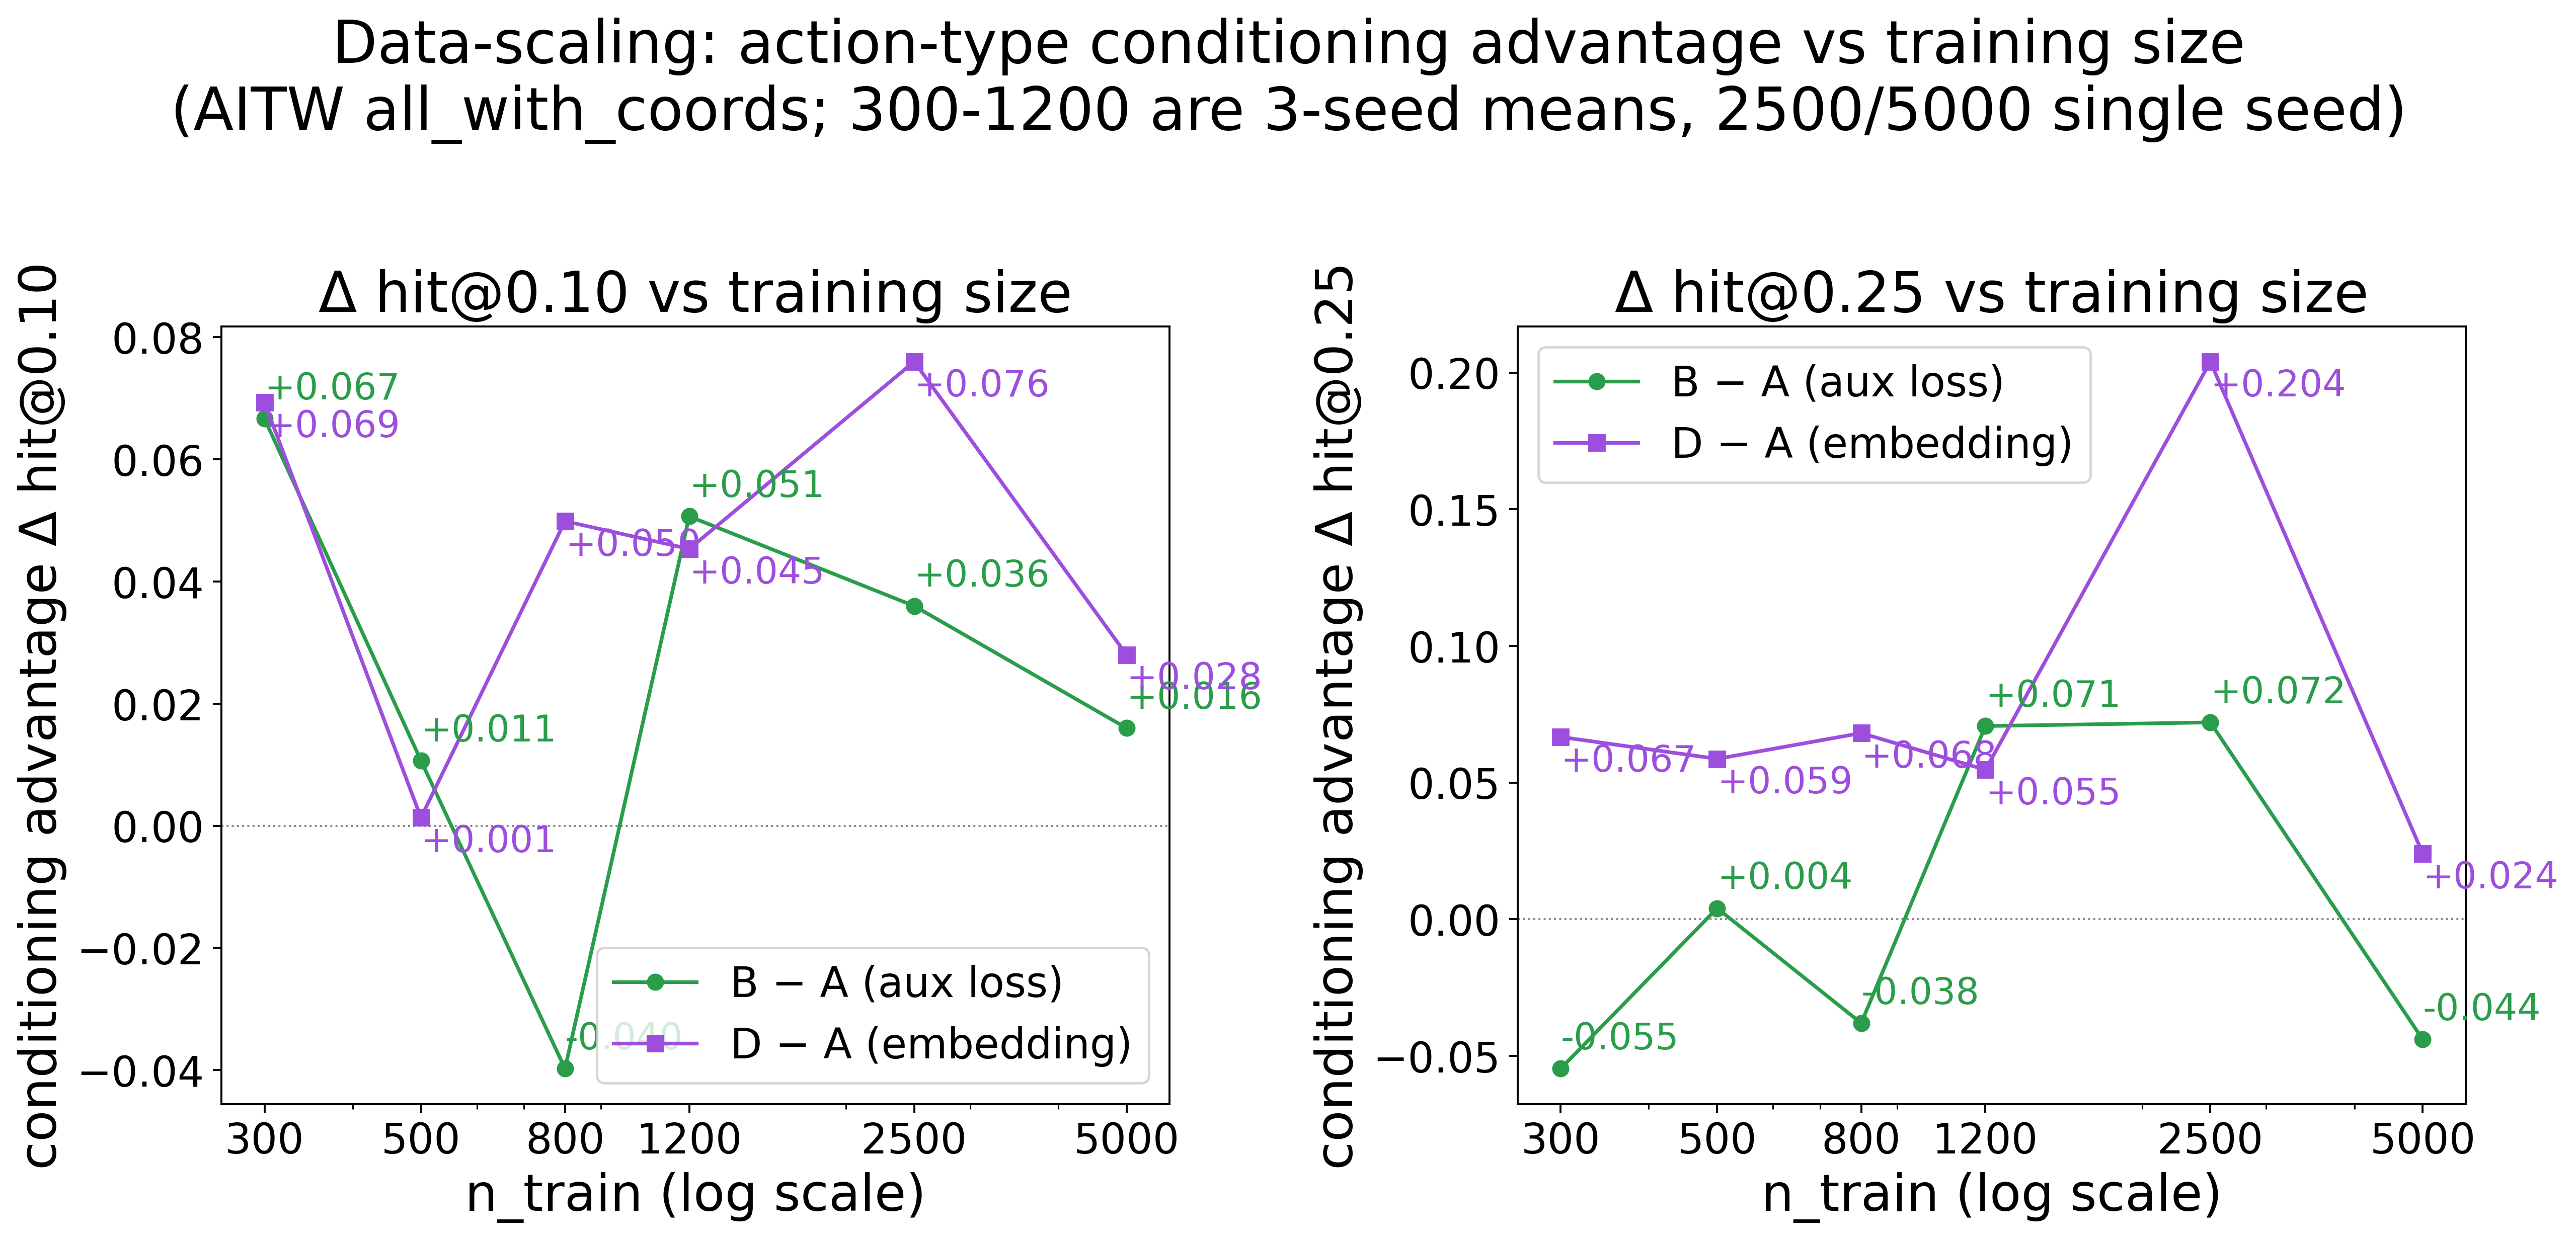
\includegraphics[width=0.98\linewidth]{figures/scaling_curve.png}
\end{center}
\caption{Conditioning advantage ($\Delta$ hit@0.10 vs.\ Variant~A) as a function of $n_{\text{train}}$, ranging from 300 to 5000. The advantage is largest at low data and shrinks with scale, confirming that action-type conditioning acts as a low-data prior that the flat baseline absorbs at scale.}
\label{fig:scaling}
\end{figure}

Figure~\ref{fig:scaling} plots the conditioning advantage $\Delta$ hit@0.10 (B $-$ A, D-hook $-$ A) across $n_{\text{train}} \in \{300, 500, 800, 1200, 2500, 5000\}$ (3 seeds for $n \leq 1200$; single seed for larger $n$).

The low-data regime ($n \in \{300, 500, 800\}$) was swept with 3 seeds each (27 runs total) specifically to test the low-data prior prediction. At $n = 300$, B and D-hook gain $+0.067$ and $+0.069$ hit@0.10 over A, respectively. At $n = 5000$, B $-$ A shrinks to $+0.016$ and hit@0.25 even reverses ($-0.044$). This \textbf{confirms the prediction} that action-type conditioning is a low-data prior that the flat baseline absorbs at scale.

D-hook is the most stable low-data mechanism: it has the best hit@0.25 and mean L2 at every low-data size, even when hit@0.10 at $n=500$ is nearly tied. B's low-data advantage exists primarily in hit@0.10 at $n=300$; it is not consistently better than D-hook in the low-data regime.

\subsection{D-Token Causal-Use Test}

\begin{table}[tb]
\begin{center}
\small
\begin{tabular}{lccc}
\toprule
Condition & hit@0.10 & hit@0.25 & mean L2 $\downarrow$ \\
\midrule
gold action id & $\mathbf{0.276}$ & $\mathbf{0.529}$ & $\mathbf{0.375}$ \\
wrong action id & $0.084$ & $0.200$ & $0.721$ \\
zeroed embedding & $0.183$ & $0.417$ & $0.492$ \\
\midrule
gold $-$ wrong & $+0.192^{**}$ & $+0.329^{**}$ & — \\
gold $-$ zero & $+0.093^{**}$ & $+0.112^{**}$ & — \\
\bottomrule
\end{tabular}
\end{center}
\caption{D-token causal-use test: D-token model evaluated with gold, wrong, or zeroed action embeddings. The learned embedding is causally used at inference — wrong/zero embeddings significantly hurt grounding. The refutation is precise: ``used but not optimal,'' not ``ignored.'' $**$: $p < 0.001$, paired bootstrap.}
\label{tab:causal}
\end{table}

If the D-token embedding were ignored at inference (a plausible explanation for its failure to beat B), swapping in the wrong action id should have no effect. Table~\ref{tab:causal} rules this out. Feeding a wrong action id collapses hit@0.10 from 0.276 to 0.084 ($-0.192$, $p < 0.001$); zeroing the embedding also hurts ($-0.093$, $p < 0.001$). The learned D-token embedding is \textbf{causally used at inference}. The refutation of D-token as the winning mechanism is therefore precise: the embedding is not inert, but it is not the best way to exploit action-type supervision compared to B's auxiliary loss or D-hook's additive conditioning.

\paragraph{Attention visualization.}
Figure~\ref{fig:attention} visualizes image-region attention for a held-out \emph{click} example under three action-type conditionings. Conditioning on the correct type concentrates more attention mass on the screenshot ($0.204$) than conditioning on \emph{type} ($0.132$) or \emph{scroll} ($0.110$), indicating that the conditioning signal reshapes where the model attends.

\begin{figure}[tb]
\begin{center}
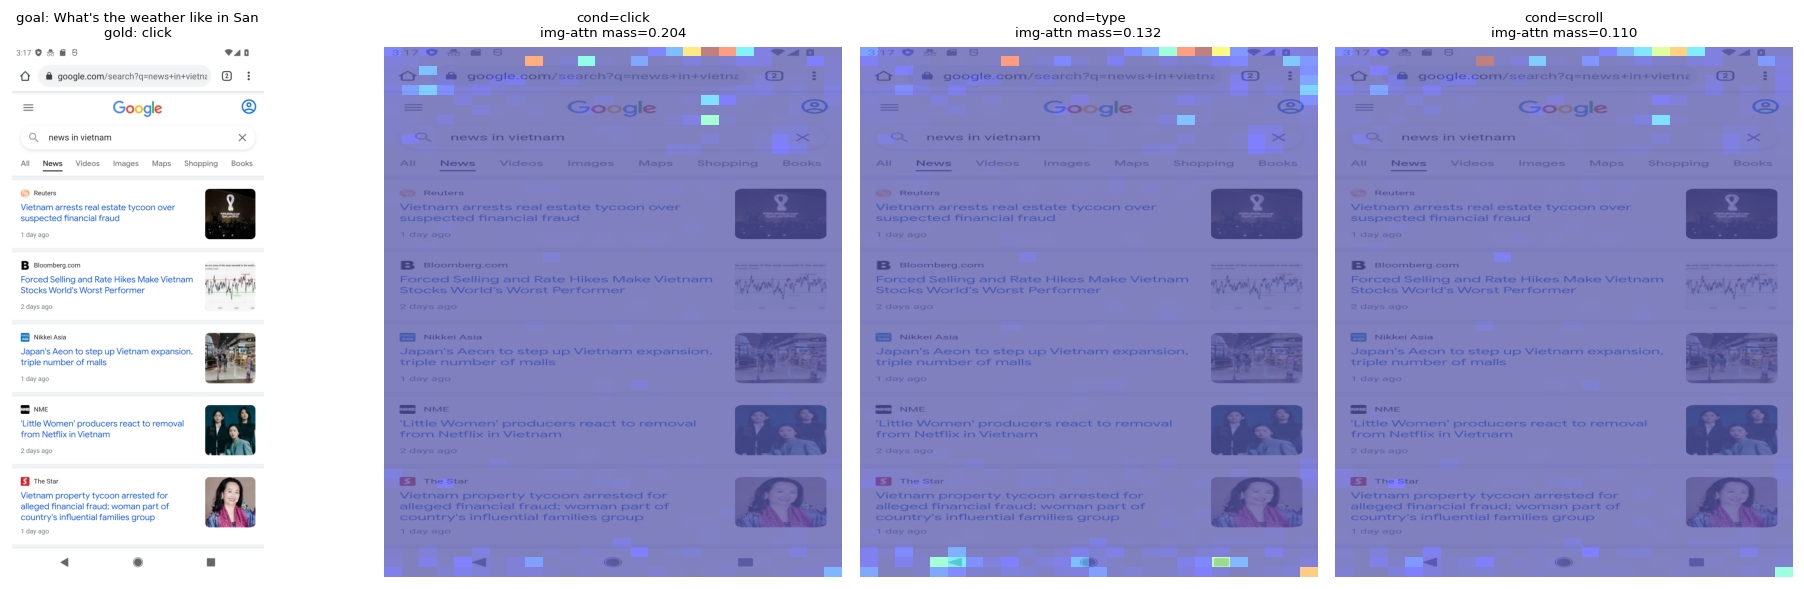
\includegraphics[width=0.98\linewidth]{figures/attn_example_1.png}
\end{center}
\caption{Image-region attention for a held-out \emph{click} example under three action-type conditionings. Conditioning on the correct type (click) places more attention mass on the screenshot ($0.204$) than conditioning on \emph{type} ($0.132$) or \emph{scroll} ($0.110$), indicating the conditioning signal reshapes spatial attention.}
\label{fig:attention}
\end{figure}

\section{Conclusion}

We studied action-type-conditioned grounding for GUI agents through a controlled five-variant ablation with paired-bootstrap significance. The main findings:

\textbf{Supported}: Factoring action-type prediction from spatial grounding significantly improves hit rates when action type is spatially informative (click-vs-scroll/type discrimination). The advantage is largest at low data and concentrated in the click class. A full two-stage pipeline with predicted types beats the flat baseline end-to-end.

\textbf{Refuted}: The specific mechanism proposed — a learned prepended action-type embedding — is not the winning approach. An auxiliary training loss (Variant B), which provides no inference-time conditioning, captures the full benefit of action-type supervision with less complexity. Stronger embedding signals (D-token, norm 2.2) compete with the image/instruction for attention rather than complement them.

\textbf{Documented}: A M-RoPE implementation pitfall where \texttt{inputs\_embeds} injection bypasses position-ID computation in Qwen2-VL, producing large false negatives that mask true model behavior.

\textbf{Mechanistic insight}: The grounding gain is click-specific disambiguation (68\% of val), not field localization. AITW \texttt{type} coordinates are degenerate, so the residual vision-grounding challenge on this dataset is click-vs-scroll/type classification, not precise text-field targeting.

\textbf{Future directions}: The auxiliary-loss finding suggests that better action-type training signal — even without explicit inference-time routing — is the more promising lever. Future work could test the conditioning advantage on ScreenSpot~\cite{seeclick} where grounding targets are diverse, and extend to larger backbones (Qwen2-VL-7B) to test whether the scaling behavior changes.

%%%%%%%%% CONTRIBUTIONS + GENAI (not counted toward the page limit)
\section*{Contributions}
\emph{[Template --- replace with your actual breakdown.]} \textbf{A.\ Chauhan}: [e.g., Stage~2 conditioning variants, Modal training/evaluation infrastructure, ablation experiments, statistical analysis, writing]. \textbf{A.\ Ilyasov}: [e.g., Stage~1 classifier, data pipeline, figures, error analysis, writing]. Both authors contributed to problem formulation, experimental design, and the final manuscript. [If all members contributed equally, state that explicitly here.]

\section*{Generative AI Usage Statement}
\emph{[Template --- verify and edit to accurately reflect your usage.]} We used generative AI tools ([tool name(s)]) as a coding and formatting aid: generating and debugging Stage~1/Stage~2 training and evaluation code, scaffolding the Modal entry points, producing figures and tables, and LaTeX formatting. All research design, hypotheses, experiments, analysis, and interpretation are our own, and we independently verified every reported number against our logged experimental results. Generative AI was not used to write the substantive analytical content of this report.

{\small
\bibliographystyle{ieee}
\bibliography{paper}
}

\end{document}
